% This LaTeX was auto-generated from MATLAB code.
% To make changes, update the MATLAB code and export to LaTeX again.

\documentclass{article}

\usepackage[utf8]{inputenc}
\usepackage[T1]{fontenc}
\usepackage{lmodern}
\usepackage{graphicx}
\usepackage{color}
\usepackage{hyperref}
\usepackage{amsmath}
\usepackage{amsfonts}
\usepackage{epstopdf}
\usepackage[table]{xcolor}
\usepackage{matlab}

\usepackage[active,tightpage]{preview}

\renewcommand{\PreviewBorder}{1in}
\newcommand{\Newpage}{\end{preview}\begin{preview}}

\sloppy
\epstopdfsetup{outdir=./}
\graphicspath{ {./Assignment_3_images/} }

\begin{document}
\begin{preview}

\matlabheadingtwo{Question a)}

\begin{par}
\begin{flushleft}
\textit{Choose appropriate initial conditions x(0|0) and P (0|0) for the filter. At t = 0 the robot head rests against a stop, which corresponds to a starting angle of (0 ± 5).}
\end{flushleft}
\end{par}

\begin{matlabcode}
clc; clear;

%% Our initial guess at the neck position.
x_post(:,1) = [0, 0, 0]';           % Put your initial estimate here. 
P_post = diag([1, 1, 10]);          % Put your initial estimate here. 


%% Run the model and plot the output of the filter
run("robot_head_1_sensor.m")

figure
labels = {"Angle \Phi","Velocity \omega","Acceleration \alpha"};
for plot_num = 1:3,
  subplot(3,1,plot_num)
  stairs(t,[x(plot_num,:); x_post(plot_num,:)]')
  ylabel([labels(plot_num)])
end

subplot(3,1,1)
legend("True", "Estimate")
subplot(3,1,3)
xlabel('Time (s)')
\end{matlabcode}
\begin{center}
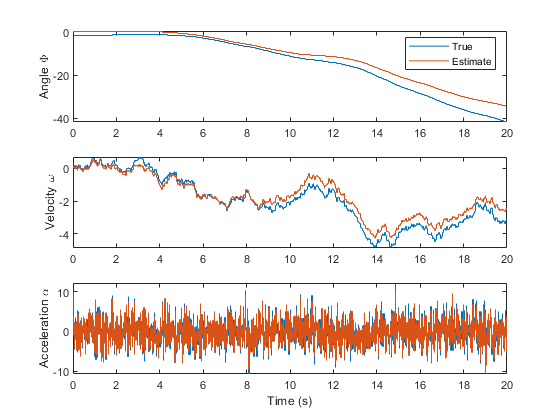
\includegraphics[width=\maxwidth{57.90265930757652em}]{figure_0.png}
\end{center}

\hrule
\matlabheadingtwo{Question b)}

\begin{par}
\begin{flushleft}
\textit{Demonstrate the start up transient of the Kalman filter by plotting L as a function of time.}
\end{flushleft}
\end{par}

\begin{matlabcode}
figure
plot(t, L_store)
xlabel("Time [s]")
ylabel("L")
title("Time series plot of kalman filter gains")
legend("L_1", "L_2", "L_3")
\end{matlabcode}
\begin{center}
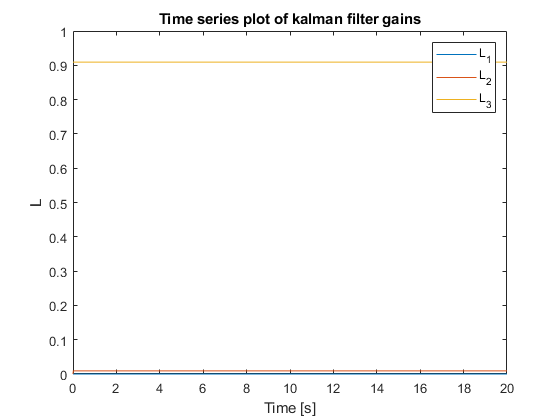
\includegraphics[width=\maxwidth{57.90265930757652em}]{figure_1.png}
\end{center}

\begin{par}
\begin{flushleft}
All kalman $L$ filter gains imeadly transition to their final position within one time step.
\end{flushleft}
\end{par}

\hrule
\matlabheadingtwo{Question c)}

\begin{par}
\begin{flushleft}
\textit{Contrast the performance of the filter with a steady state Kalman filter. You should use Matlab to design the steady state Kalman gain.}
\end{flushleft}
\end{par}

\begin{matlabcode}
%% Store the steady state L as the previously converged L
L_s = L;
x_post_s(:,1) = [0, 0, 0]';

%% Run a new verion of the model that calculate both the time variant and time invariant kalman filters
run("robot_head_steady_state.m")

%% Plot the new filter outputs against the actual output
figure
labels = {"Angle \Phi","Velocity \omega","Acceleration \alpha"};
for plot_num = 1:3,
  subplot(3,1,plot_num)
  stairs(t,[x(plot_num,:); x_post(plot_num,:); x_post_s(plot_num,:)]')
  ylabel([labels(plot_num)])
end
subplot(3,1,1)
legend("True", "Time Variant L", "Time Invariant L")
subplot(3,1,3)
xlabel('Time (s)')
\end{matlabcode}
\begin{center}
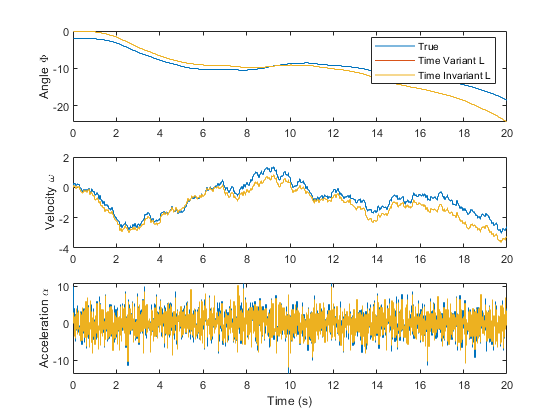
\includegraphics[width=\maxwidth{57.90265930757652em}]{figure_2.png}
\end{center}

\begin{par}
\begin{flushleft}
It can be seen from this simulation that the steady state kalman filter is idential to the time invariant one. This is expected based on the plotting of the original kalman filter's L gains, as they step imedatly to their final states. 
\end{flushleft}
\end{par}

\hrule
\matlabheadingtwo{Question d)}

\begin{par}
\begin{flushleft}
\textit{Add sensor two to the system and demonstrate its effect on the state estimate. Contrast the tracking performance with and without the extra sensor for a variety of initial conditions (that is consider examples of initial estimates that are both near and far from the robot’s true state).}
\end{flushleft}
\end{par}

\begin{matlabcode}
clc; clear;

for estimate = [0, 10, 50]
    x_estimate = [estimate, 0, 0]';
    p_estimate = [1, 1, 1];
    
    %% Run the single sensor model and plot the output of the filter
    x_post(:,1) = x_estimate;       % Put your initial estimate here. 
    P_post = diag(p_estimate);       % Put your initial estimate here. 
    run("robot_head_1_sensor.m")
    
    figure
    labels = {"Angle \Phi","Velocity \omega","Acceleration \alpha"};
    for plot_num = [1, 3, 5],
      subplot(3,2,plot_num)
      stairs(t,[x(ceil(plot_num/2),:); x_post(ceil(plot_num/2),:)]')
      ylabel([labels(ceil(plot_num/2))])
    end
    
    %% Run the single sensor model and plot the output of the filter
    x_post(:,1) = x_estimate;       % Put your initial estimate here. 
    P_post = diag(p_estimate);       % Put your initial estimate here.
    run("robot_head_2_sensor.m")
    
    for plot_num = [2, 4, 6],
      subplot(3,2,plot_num)
      stairs(t,[x( plot_num/2,:); x_post(plot_num/2,:)]')
    end
    
    %% Add titles and axis
    subplot(3,2,1)
    legend("True", "Estimate")
    title("Single Sensor")
    subplot(3,2,2)
    legend("True", "Estimate")
    title("Dual Sensor")
    subplot(3,2,5)
    xlabel("Time [s]")
    subplot(3,2,6)
    xlabel("Time [s]")
    sgtitle(['\Phi Initial Estimate = ' num2str(estimate)])
end
\end{matlabcode}
\begin{center}
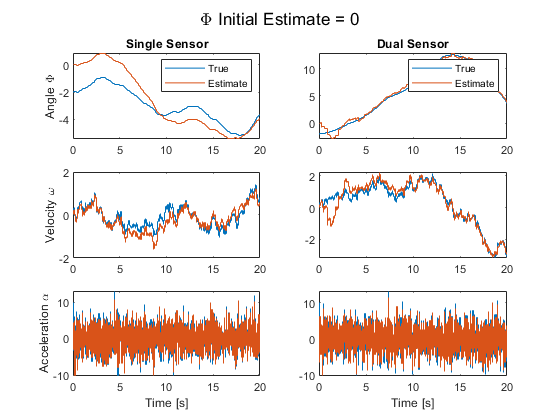
\includegraphics[width=\maxwidth{57.90265930757652em}]{figure_3.png}
\end{center}
\begin{center}
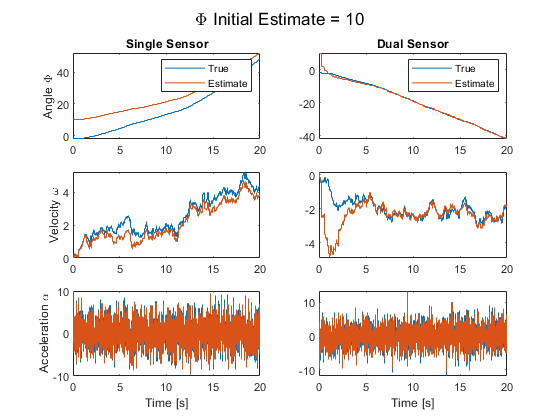
\includegraphics[width=\maxwidth{57.90265930757652em}]{figure_4.png}
\end{center}
\begin{center}
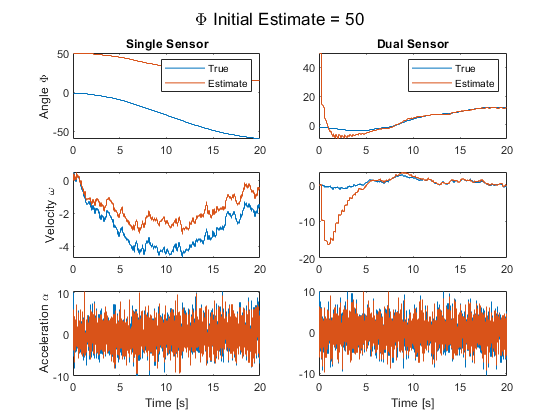
\includegraphics[width=\maxwidth{57.90265930757652em}]{figure_5.png}
\end{center}

\begin{par}
\begin{flushleft}
From the plots above it can be seen that the two sensor Kalman filter is far superior at tracking the true states of the system. It can also be seen that for all initial estimates, the multi-sensor system managed to return to the true value of the system.
\end{flushleft}
\end{par}

\hrule
\matlabheading{Question e)}

\begin{par}
\begin{flushleft}
\textit{Modify your code to include validation gating of some form and demonstrate it working by injecting occasional errors into the measurement stream. Be sure to explain your technique. }
\end{flushleft}
\end{par}

\begin{matlabcode}
clc; clear;

%% Our initial guess at the neck position.
x_post(:,1) = [0, 0, 0]';           % Put your initial estimate here. 
P_post = diag([1, 1, 10]);          % Put your initial estimate here. 

run("robot_head_2_sensor_no_gate.m")

figure
labels = {"Angle \Phi","Velocity \omega","Acceleration \alpha"};
for plot_num = 1:3,
  subplot(3,1,plot_num)
  stairs(t,[x(plot_num,:); x_post(plot_num,:)]')
  ylabel([labels(plot_num)])
end

subplot(3,1,1)
legend("True", "Estimate")
subplot(3,1,3)
xlabel('Time (s)')
sgtitle("No Validation Gating")
\end{matlabcode}
\begin{center}
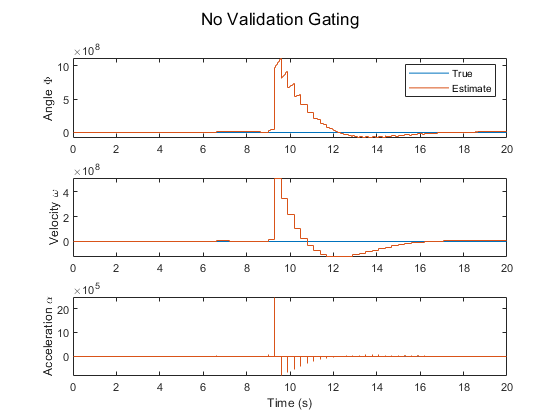
\includegraphics[width=\maxwidth{56.196688409433015em}]{figure_6.png}
\end{center}
\begin{matlabcode}

%% Our initial guess at the neck position.
x_post(:,1) = [0, 0, 0]';           % Put your initial estimate here. 
P_post = diag([1, 1, 10]);          % Put your initial estimate here. 

run("robot_head_2_sensor_gate.m")

figure
labels = {"Angle \Phi","Velocity \omega","Acceleration \alpha"};
for plot_num = 1:3,
  subplot(3,1,plot_num)
  stairs(t,[x(plot_num,:); x_post(plot_num,:)]')
  ylabel([labels(plot_num)])
end

subplot(3,1,1)
legend("True", "Estimate")
subplot(3,1,3)
xlabel('Time (s)')
sgtitle("Validation Gating")
\end{matlabcode}
\begin{center}
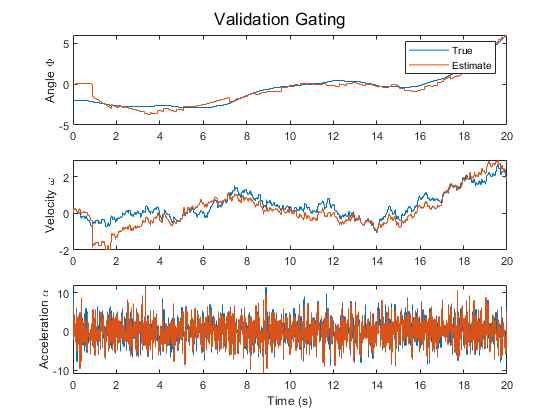
\includegraphics[width=\maxwidth{56.196688409433015em}]{figure_7.png}
\end{center}

\begin{par}
\begin{flushleft}
The validation gating was done by looking at the ratio of the previous estemate to the current measurment. If this ratio was greater or smaller than some given threshold, the new measurment was replaced with the previous estemate. 
\end{flushleft}
\end{par}

\begin{par}
\begin{flushleft}
This was then tested by injecting measurment errors into the system, multiplying the measurment by a large random number. 
\end{flushleft}
\end{par}
\end{preview}
\end{document}
